\newpage
\section{CMSSW and Fireworks (cmsShow) (08/11/2016)}
\label{sec:fireworks}

CMS SoftWare (CMSSW) is software that CMS physicists can access to perform analyses, etc. The GitHub repository is located at \url{https://github.com/cms-sw/cmssw}. If I want to set up a CMSSW environment, I need to type the commands

\begin{lstlisting}[belowskip=-0.7cm, language=sh, numbers=none]
ssh ebhal@lxplus.cern.ch # or whatever remote server I'm logging in to
cmsrel CMSSW_7_6_3 # Only need to do this once. Can also change version I'm working with
cd CMSSW_7_6_3/src
cmsenv
\end{lstlisting}

and I can follow the instructions in \ref{sec:cutflowtablesSUS15005} to use the different modules and packages it contains. CMSSW can be used to access and analyse data and Monte Carlo, as well as simulate the latter. If I want to use \madgraph\ or \madanalysis\ or something on Soolin, I need to execute the commands above (or put them in a script and \verb!source! it) before using the programs. There's also a software component called Fireworks (or cmsShow) which is an event-display project, i.e., it displays a visualisation of the events from a ROOT file. It shows particle tracks and other information confined within the detector/simulation. More information can be found at \url{https://twiki.cern.ch/twiki/bin/view/CMSPublic/WorkBookFireworks}.

To use Fireworks, download it using the instructions in the above link. Then navigate to the directory \textbf{cmsShow-$<$version$>$/} and type

\verb!./cmsShow <name of root file>!

The example file \textbf{data.root} gives this output:

\begin{figure}[H]
\centering
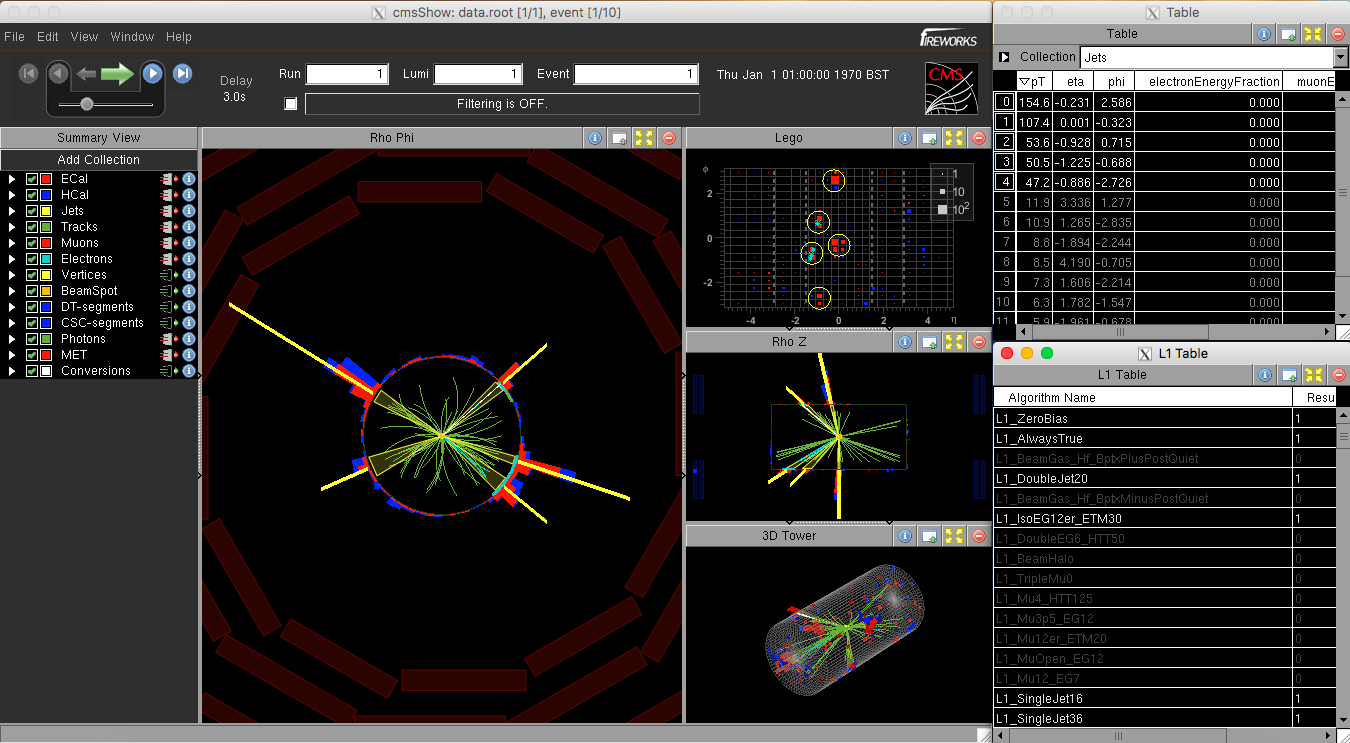
\includegraphics[width=\textwidth]{./sec12/fireworksexample.png}
\caption{The Fireworks interface using the example root file provided by the program (data.root). This program provides a visualisation of the particle tracks and detector information (and probably various tools that I haven't explored yet).}
\end{figure}

